\documentclass[a4paper, 12pt]{scrartcl}
\usepackage[utf8]{inputenc}
\usepackage[ngerman]{babel}
\usepackage[T1]{fontenc}
\usepackage{graphicx}
\usepackage{hyperref}

\hypersetup{
	colorlinks=true,
	linkcolor=blue,
	filecolor=blue,      
	urlcolor=blue,
	pdftitle={ Example},
	pdfpagemode=FullScreen,
}

\title{End-2-End-Prozess}
\titlehead{Praxisbericht}
\author{Maksym Mykhailych}
\date{09. September 2025}

\begin{document}
	\maketitle
	\newpage
	\section*{Abstract}
	\newpage 	
	\tableofcontents
	\newpage
	
	\newpage
	\section{Einleitung}
	Einleitender Text.
	\newpage
	\subsection{Motivation}
	\subsection{Aufgabenstellung}
	\subsection{Aufbau der Arbeit}
	Text.
	\newpage
	\section{Grundlagen}
	\subsection{Vorstellung von Capgemini}
	\subsubsection{Gesamtheitliche Darstellung von Capgemini} %VOrstellung von Capgemini(Geschichte, Zahlen, Wie groß?)
Capgemini, mit Hauptsitz in Paris, ist ein transnationales, börsennotiertes Unternehmen, das Beratungs-, Technologiedienstleistungen und digitale Transformationslösungen anbietet. Das Unternehmen bietet eine Vielzahl von Dienstleistungen, darunter Beratung, Technologie und Outsourcing. Mit einer Präsenz in über 50 Ländern bedient Capgemini Kunden aus diversen Branchen, einschließlich Finanzdienstleistungen, Automobilindustrie, Gesundheitswesen und Einzelhandel. Im \href{https://www.capgemini.com/de-de/news/pressemitteilung/capgemini-delivers-another-record-performance-in-2023/}{Jahr 2023} erzielte Capgemini einen Umsatz von 22,5 Milliarden Euro und beschäftigt weltweit etwa 340.000 Mitarbeiter, davon rund 12.500 in Deutschland laut der internen Daten.
	\begin{figure}[h!]
		\begin{center}
			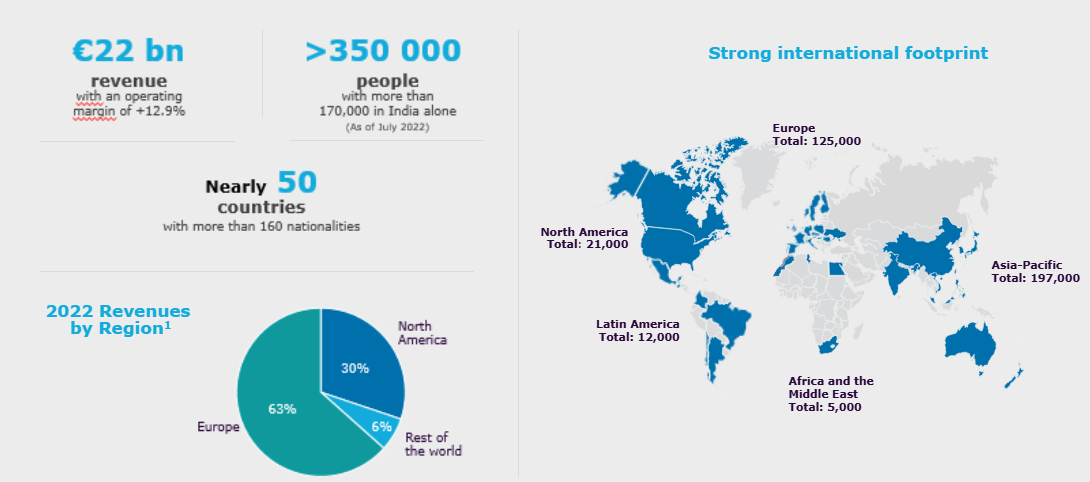
\includegraphics[width=12cm]{CApgemini zahlen.png}
			\caption{Stand von Capgemini zu 2023}
			\label{Stand von Capgemini}
		\end{center}
	\end{figure}
	\subsubsection{Struktur und Organisation in Deutschland}

Capgemini Gruppe bietet ihren Kunden eine End-to-End-IT-Transformation, die von der Umgestaltung komplexer IT-Architekturen bis hin zur Entwicklung spezifischer kleiner Funktionen reicht. In diesem Zusammenhang verfügt Capgemini über große Mitarbeiteranzahl und besteht aus mehreren \href{https://www.capgemini.com/de-de/unternehmen/wer-wir-sind/unsere-marken/}{ Marken}:
	\begin{itemize}
		\item \textbf{Capgemini:} Das Mutterunternehmen bietet ein breites Spektrum an Dienstleistungen, darunter IT-Beratung und Technologie-Services.
		
		\item \textbf{Capgemini Invent:} Diese Sparte konzentriert sich auf die strategische digitale Entwicklung der Kunden.
		\item \textbf{Capgemini Engineering:} Ein weltweit führender Anbieter von Engineering- und F\&E-Dienstleistungen, der Kunden dabei unterstützt, ihren Weg zur Intelligent Industry zu beschleunigen.
		\item \textbf{Sogeti:} Entwickelt, testet und schützt innovative Anwendungen für Unternehmen und stützt sich dabei auf Expertise in den Bereichen Beratung, Testen, agile und Cloud-Entwicklung sowie Cybersicherheit.
	\end{itemize}
Dies sind die wichtigsten Marken von Capgemini in Deutschland. Meine Erfahrung habe ich im Mutterunternehmen von Capgemini gesammelt, wo das Unternehmen auch intern in verschiedene Abteilungen unterteilt ist. Meine Tätigkeit fand in der Abteilung statt, die paketbasierte Lösungen %Im glossar erklären was PBS ist(SAP, Windchill etc.)
  für Kunden anbietet.


	\newpage
	\subsection{Definition des End-2-End-Prozesses}
Ein End-to-End-Prozess(End-2-End) bezeichnet den Ablauf einer Aktion vom Anfang bis zum logischen Ende. Es gibt verschiedene End-to-End-Prozesse, die in Unternehmen betrachtet werden können. Zum Beispiel ist im Bereich Human Resources der sogenannte Hire-to-Retire-Prozess relevant, in der Logistik der Supply-Chain-Prozess und im Bereich des Product Lifecycle Management (PLM) der End-to-End-Prozess des Produktlebenszyklus.
	\subsubsection{Überblick des allgemeinen End-2-End-Prozesses} %wie sieht algemein E2E-Prozess bei der Beratung!
%Wie bei allen Unternehmen ist die Hauptaufgabe der Consultingsunternehmen, den eigenen Unsatz und das Gewinn jährlich zu steigern. 
In dieser Arbeit wird der gesamte Prozess des Projektmanagements betrachtet. Das Projektmanagement besteht üblicherweise aus fünf auf Abbildung \ref{Projektmanagment} gezeigten Phasen\cite{timinger2024modernes}
	\begin{figure}[h!]
		\begin{center}
			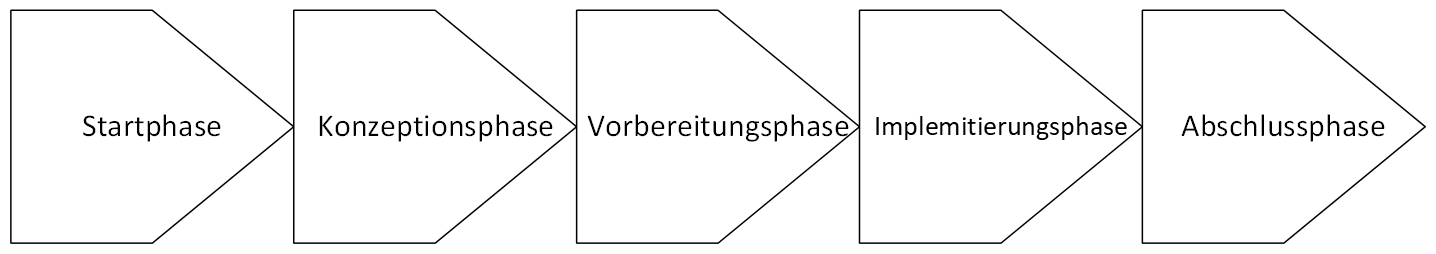
\includegraphics[width=12cm]{Drawing.png}
			\caption{Phasenplan\cite{timinger2024modernes}}
			\label{Projektmanagment}
		\end{center}
		
	\end{figure}
	\begin{enumerate}
		\item \textbf{Startphase:} 
In dieser Phase erfolgt die Initiierung des Projekts, wobei die grundlegenden Ziele und Anforderungen, Nachfrage definiert werden. Die strategische Ausrichtung des Projekts wird durch die Fachbereichsleiter sowie die Stakeholder festgelegt.
		\item \textbf{Konzeptionsphase:}
Auf Grundlage der definierten Ziele entwickeln die Fachbereichsleiter (z. B. die Leiter der Abteilungen IT, Ressourcenmanagement und HR) detaillierte Pläne und Konzepte zur Umsetzung des Projekts. In diesem Rahmen wird bestimmt, welche Mitarbeiter und Materialien erforderlich sind. Zudem wird überprüft, ob das Unternehmen über die benötigten Fachkräfte verfügt oder ob eine externe Rekrutierung notwendig ist.
		\item \textbf{Vorbereitungsphase:} 
In dieser Phase werden die für die Projektdurchführung erforderlichen Ressourcen und Materialien beschafft sowie die organisatorischen Strukturen eingerichtet. Dabei übernehmen insbesondere der Projektleiter, das Beschaffungsteam und die Fachbereichsleiter eine zentrale Rolle, indem sie sicherstellen, dass alle notwendigen Ressourcen bereitgestellt werden.
		\item \textbf{Implementierungsphase:}  
Die Umsetzung des Projekts erfolgt gemäß den zuvor entwickelten Plänen und Konzepten. Während dieser Phase überwachen der Projektleiter, das Projektteam und die Qualitätssicherung den Fortschritt, um die termingerechte und qualitativ hochwertige Durchführung der Maßnahmen sicherzustellen.
		\item \textbf{Abschlussphase:} 
Nach der Umsetzung wird das Projekt formal abgeschlossen. Dabei erfolgt eine Bewertung der Ergebnisse, und die Projektdokumentation wird erstellt. Zudem wird ein Plan zur Vermarktung des Produkts entwickelt, um eine effiziente Markteinführung und einen erfolgreichen Vertrieb sicherzustellen. Der Projektleiter, das Projektteam sowie die Stakeholder sind maßgeblich an der Evaluierung der Projektergebnisse, der Erstellung der Dokumentation und der Entwicklung der Verkaufsstrategie beteiligt.
	%REFERENZIEREN
	\end{enumerate}
Jedes Projekt unterscheidet sich in Zielen, Inhalten und Dauer. Dennoch ist der Projektablauf meist ähnlich strukturiert. Typischerweise umfasst er die folgenden Phasen: Initiierung, Planung, Durchführung, Überwachung und Abschluss. Diese allgemeinen Phasen ermöglichen eine systematische und effiziente Projektabwicklung, unabhängig von den spezifischen Unterschieden zwischen den Projekten\cite{wegmann2006projektmanagement}.
	\subsubsection{End-2-End-Prozess bei Capgemini}
Capgemini ist zwar ein Beratungsunternehmen, das keine eigenen Produkte entwickelt, sondern andere Unternehmen unterstützt. Aus diesem Grund unterscheidet sich das Projektmanagement und die Projektphasen von denen in Industrieunternehmen. In Abbildung \ref{Projektmanagment_Campgeini} sind die folgenden 6 Projektphasen definiert \cite{wegmann2006projektmanagement}:
	\begin{figure}[h!]
		\begin{center}
			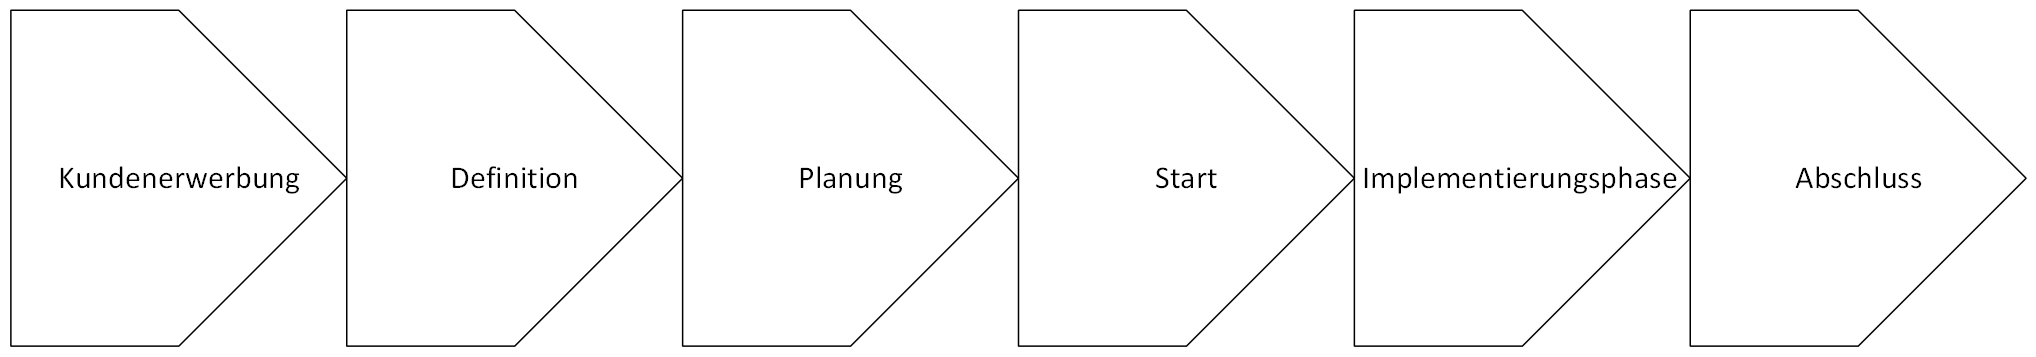
\includegraphics[width=12cm]{Projektmanagement_Capgemini .png}
			\caption{Phasenplan bei der Beratungsunternehmen \cite{wegmann2006projektmanagement}}
			\label{Projektmanagment_Campgeini}
		\end{center}
	\end{figure}
	\begin{enumerate}
	\item \textbf{Kundengewinnung:} In dieser Phase bemüht sich die Vertriebsabteilung von 		Capgemini, neue Projekte zu akquirieren. Dabei werden verschiedene Strategien eingesetzt, wie die Demonstration der Fachkompetenz von Capgemini in relevanten Bereichen, die Hervorhebung erfolgreicher Referenzprojekte und die Präsentation von Innovationen auf Messen. Zusätzlich werden potenzielle Kunden durch gezielte Marketingmaßnahmen und persönliche Kontakte angesprochen, um das Vertrauen in die Fähigkeiten von Capgemini zu stärken.
	\item \textbf{Definition:} In dieser Phase versucht Capgemini, den Bedarf des
	Unternehmens zu definieren. Außerdem wird der Vertrag diskutiert und ausgearbeitet, um die Rahmenbedingungen und Erwartungen klar festzulegen.

	\item \textbf{Planung:} In dieser Phase wird das Projekt detailliert geplant. Es wird 
	festgelegt, wie viel Zeit für die Durchführung des Projekts benötigt wird und welche Rollen und Ressourcen erforderlich sind. Das Staffing-Team wählt entsprechend qualifizierte Mitarbeiter aus, um die Projektanforderungen zu erfüllen.
	\item \textbf{Start:} In dieser Phase versucht das gebildete Team, das Problem zu definieren und eine ausführliche Lösung zu erarbeiten. Dies umfasst die Erstellung eines detaillierten Zeitplans sowie die Festlegung der Verantwortlichkeiten für die einzelnen Aufgaben.
	\item \textbf{Implementierungsphase:} Dies ist die zeitlich umfangreichste Phase, in der alle Pläne in die Realität umgesetzt werden. Jeder Mitarbeiter führt seine spezifischen Aufgaben aus, um die Projektziele zu erreichen.
	\item \textbf{Abschluss} Auch als sogenannte Abschlussphase bekannt, in der alle organisatorischen und finanziellen Fragen zwischen dem Unternehmen und Capgemini geklärt werden.
	\end{enumerate}
	\subsection{PLM-Systeme}
	Das Auto ist heutzutage ein unverzichtbarer Begleiter des Menschen, der ihn bei der schnellen Fortbewegung unterstützt. Aus der Sicht eines Ingenieurs jedoch ist es auch eine komplexe Maschine, die aus Hunderttausenden von Einzelteilen besteht, die effizient verwaltet werden müssen. In diesem Zusammenhang entstand zu Beginn des 21. Jahrhunderts ein neues Paradigma in Fertigungsunternehmen: das Product Lifecycle Management (PLM). PLM ermöglicht es Unternehmen, ihre Produkte während des gesamten Lebenszyklus zu überwachen und zu steuern. Das ist eine der wichtigsten Aktivitäten der Fertigungsunternehmen\cite{stark2011product}.
	\subsubsection{Allgemeine Übersicht der PLM-Systeme}
	
	\begin{figure}[h!]
		\begin{center}
			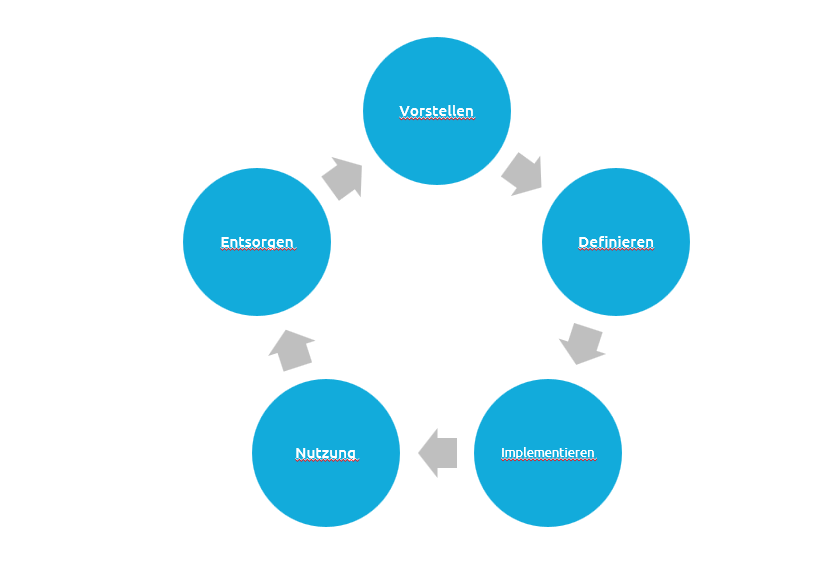
\includegraphics[width=12cm]{PLM.png}
			\caption{ Product Lifecycle Management}
			\label{PLM}
		\end{center}
	\end{figure}


	\subsubsection{Vorstellung von verschiedenen Vendoren}
jv mn 
	\newpage
	\section{Durchführung}
	\subsection{Phase 1: Sales} 
	\subsubsection{Ausgangslage und Aufgabenstallung} %Ich beschäftige mich mit der Showcase für die Kunden um das Projekt zu kriegen.
	\subsubsection{Anforderungen für die Erstellung der Demonstratorenübersicht} %welche versionen die Demonstratoren haben, Ziel des Demonstrators, Beschreibungen etc.
	\subsubsection{Tools-Analyse}%Welche Tools gibt und welche sind geeignet für meinen Demostrator(Beschränung von Unternehmen betrachten)
	\subsubsection{Erstellung der Demonstratorenübersicht}
	\newpage
	\subsection{Phase 2: Staffing}
	\subsubsection{Relevanz der Staffing für Capgemini}%was lebenswichtiges macht Christoph
	\subsubsection{Ausgangslage und Aufgabenstellung}
	\subsubsection{Anforderungen fürs Reporting}
	\subsubsection{Umsetzung des Berichtswesen...}
	\newpage
	\subsection{Phase 3: Projektplanung}
	\newpage
	\subsection{Phase 4: Delivery}
	\newpage
	\subsection{Phase 5: Closure}
	\newpage
	\section{Auswertung}
	\subsection{Validierung der Anforderung}%für PLM
	\newpage
	\section{Ergebnisse und Diskussion}
		\newpage
	\section{Ausblick}

		\newpage
	\section{Anhang}
	\bibliography{Reference.bib}
\end{document}